% Provenance (never printed): see sources/outline_sources.md (Year 1: hotspots and
% mantle plumes; hotspot chains and absolute plate motion; large igneous provinces).
% Hotspot map, pole fit, rates and swell from figdata/bachelor-1/hotspots.py (data
% data/derived/bachelor-1-hotspots.csv, Table 1 of the Morgan and Morgan 2007 electronic
% supplement); exercise and problem values in the Book 3 scratch calculators calc/ch15.py and
% calc/ch15ex.py. "Hotspot" is re-founded from Book 1 (g7 volcanoes), "hotspot track"
% from Book 2 (g11 plate-motions); Book 2 owns the age--distance fit of the Hawaiian
% chain, so this chapter fits the Pacific Euler pole from track directions instead.
\chapter{热点与板内火山作用}\label{ch:b1:hotspots}

自 1983 年 1 月起并在此后数十年间，夏威夷岛上的基拉韦厄火山
几乎不曾停歇地从其东裂谷带上的一个火山口喷发，
Pu\textquoteleft u~\textquoteleft O\textquoteleft o 火口，每年喷出约
\qty{0.12}{km^3} 的熔岩。基拉韦厄火山位于太平洋板块中部，
离任何洋中脊或\omterm{def:b1:active-margins:active-margin}{海沟}都有数千千米。向西北，
夏威夷群岛的岛屿越来越老，随后没入海面之下，
此后岛链仍以一列沉没的火山延伸数千千米。
板块构造可以解释板块边界处的火山；本章讨论的则是它不能直接解释的火山——\omterm{def:b1:hotspots:hotspot}{热点}，
以及\omterm{def:b1:hotspots:hotspot}{热点}反过来能告诉我们的东西：板块如何在深部\omterm{def:b1:layered-earth:layers}{地幔}之上运动，
有多少热量和岩石从下方上涌，
以及少数规模巨大的熔岩喷溢，
即\omterm{def:b1:hotspots:lip}{大火成岩省}，是如何形成的。
% ledger: pp1801:kilauea-rate

\begin{recall}
\omterm{def:b1:hotspots:hotspot}{热点}从\omterm{def:b1:layered-earth:layers}{地幔}深部为火山供给岩浆，而板块在其上方运动，
板块则带走一条\omterm{def:b1:hotspots:track}{热点轨迹}，轨迹上的火山
离\omterm{def:b1:hotspots:hotspot}{热点}越远越老（第 1 册，七年级；第 2 册，十一年级）。绕\omterm{def:b1:plate-kinematics:euler-pole}{欧拉
矢量} $\vec\omega$ 转动的板块以 $\vec v = \vec\omega\times\vec r$ 运动，
速率为 $\omega R\sin\Delta$，方向垂直于连接该点与
\omterm{def:b1:plate-kinematics:euler-pole}{欧拉极}的\omterm{def:b1:spherical-astronomy:spherical-triangle}{大圆}（见\cref{ch:b1:plate-kinematics}）；地形起伏由\omterm{def:b1:isostasy-gravity:isostasy}{地壳均衡}支撑
（见\cref{ch:b1:isostasy-gravity}）；温热的岩石密度较小，
相对减小的比例为 $\alpha\,\Delta T$（见\cref{ch:b1:rifts-ridges-margins}）。
\end{recall}

\section{热点与地幔柱}\label{sec:b1:hotspots:plumes}

\begin{definition}[热点]\label{def:b1:hotspots:hotspot}
称\emph{热点}\index{热点}为一个火山活动区，其位置
不依赖于板块边界，持续活动数千万年，
并被认为由比周围\omterm{def:b1:layered-earth:layers}{地幔}更热的\omterm{def:b1:layered-earth:layers}{地幔}物质供给。
\end{definition}

\omterm{def:b1:hotspots:hotspot}{热点}有多少个，取决于如何计数。本章所用的\omterm{def:b1:hotspots:hotspot}{热点}表
列有 68 个\omterm{def:b1:hotspots:hotspot}{热点}，但编者剔除了若干他们认为不能记录板块运动的特征，
并将其中部分保留下来的\omterm{def:b1:hotspots:hotspot}{热点}仅定为“可能”\omterm{def:b1:hotspots:hotspot}{热点}；
有些\omterm{def:b1:hotspots:hotspot}{热点}，例如夏威夷、冰岛和留尼汪，
轨迹长而规则，产出量大，这与来自深部源区的特征相符；
其他\omterm{def:b1:hotspots:hotspot}{热点}则规模小、寿命短。多数\omterm{def:b1:hotspots:hotspot}{热点}火山喷发玄武岩；
若\omterm{def:b1:hotspots:hotspot}{热点}位于大陆之下，高温玄武岩会熔化\omterm{def:b1:layered-earth:layers}{地壳}，
而大规模喷发转为流纹岩，黄石即为一例。
% ledger: mm07:table, data:b3-hotspots, yvo:calderas

\begin{definition}[地幔柱]\label{def:b1:hotspots:plume}
称\emph{地幔柱}\index{地幔柱}为一股炽热而具浮力的\omterm{def:b1:layered-earth:layers}{地幔}岩石柱，
自\omterm{def:b1:layered-earth:layers}{地幔}深部的\omterm{def:b1:heat-budget:boundary-layer}{热边界层}上升。新生\omterm{def:b1:layered-earth:layers}{地幔}柱具有一个
大而膨胀的\emph{柱头}，下接一条细长的\emph{柱尾}，即通道；一旦
柱头在\omterm{def:b1:layered-earth:lithosphere}{岩石圈}之下铺展开来，柱尾便持续向地表输送熔体，
长达数千万年。
\end{definition}

这一形状来自实验室。1970 年代的水槽实验中，一层
较轻、黏度低于其上方流体的一层流体，以圆形团块的形式上升，
后方由一根管道供给，形如蘑菇。抵达\omterm{def:b1:layered-earth:lithosphere}{岩石圈}底部的\omterm{def:b1:hotspots:plume}{地幔柱}柱头
向四周铺展并变扁；压力下降，炽热的
岩石大量熔融。溢流玄武岩与此图景相符：其火山活动
持续约千万年，但其大部分体积是在约
百万年甚至更短的时间内喷出，它们常与大陆的裂解相伴，
（见\cref{sec:b1:hotspots:lips}）。
% ledger: hist:plumes (Whitehead and Luther 1975), cr03:summary

\begin{omfigure}
\begin{tikzpicture}[font=\scriptsize,
  lbl/.style={fill=white, fill opacity=0.8, text opacity=1, inner sep=1pt, align=center}]
% ---- panel (a): the head arrives ----
\begin{scope}
\clip (0,-5) rectangle (6.4,1.3);
\fill[orange!12] (0,-5) rectangle (6.4,0);
\fill[omSea!45] (0,0) rectangle (6.4,0.55);
\fill[omLithBasalt!55] (0,0) rectangle (6.4,-0.9);
% flood basalt: a stack of flat flows on the sea floor
\fill[black!55] (2.5,0) -- (2.7,0.32) -- (6.1,0.32) -- (6.3,0) -- cycle;
\foreach \y in {0.08,0.16,0.24} \draw[white!70!black, line width=0.3pt] (2.62,\y) -- (6.18,\y);
% plume: tail and flattened head
\fill[red!40] (4.25,-5) -- (4.25,-1.7) -- (4.55,-1.7) -- (4.55,-5) -- cycle;
\fill[red!40] (4.4,-1.45) ellipse[x radius=1.9, y radius=0.55];
\draw[red!60!black, line width=0.4pt] (4.25,-5) -- (4.25,-1.95) (4.55,-5) -- (4.55,-1.95);
\draw[red!60!black, line width=0.4pt] (4.4,-1.45) ellipse[x radius=1.9, y radius=0.55];
% melt rising through the plate
\foreach \x in {3.2,3.9,4.6,5.3}
  \draw[red!75!black, line width=0.6pt, decorate, decoration={snake, amplitude=0.6pt, segment length=3pt}] (\x,-1.1) -- (\x,0.05);
\end{scope}
\draw[black!70] (0,-5) rectangle (6.4,1.3);
\node[lbl, anchor=north west] at (0.1,1.25) {(a) 柱头抵达};
\node[lbl, anchor=west] at (0.1,-0.45) {岩石圈};
\node[lbl, anchor=west] at (0.1,0.3) {海};
\node[lbl, anchor=south] at (4.4,0.62) {溢流玄武岩（LIP）};
\node[lbl, anchor=east] (ph) at (1.9,-1.75) {柱头};
\draw[black!70] (ph.east) -- (2.7,-1.6);
\node[lbl, anchor=east] at (4.1,-3.6) {柱尾};
\node[lbl, anchor=west] at (0.1,-4.6) {地幔};
% ---- panel (b): the plate has moved on ----
\begin{scope}[xshift=6.8cm]
\begin{scope}
\clip (0,-5) rectangle (6.4,1.3);
\fill[orange!12] (0,-5) rectangle (6.4,0);
\fill[omSea!45] (0,0) rectangle (6.4,0.55);
\fill[omLithBasalt!55] (0,0) rectangle (6.4,-0.9);
% the flood basalt, carried away to the left
\fill[black!55] (-0.9,0) -- (-0.7,0.32) -- (1.0,0.32) -- (1.2,0) -- cycle;
\foreach \y in {0.08,0.16,0.24} \draw[white!70!black, line width=0.3pt] (-0.8,\y) -- (1.08,\y);
% the chain: older volcanoes to the left, lower (they sank as the plate cooled)
\fill[black!35] (1.45,0) -- (1.75,0.2) -- (2.05,0) -- cycle;
\fill[black!38] (2.15,0) -- (2.5,0.3) -- (2.85,0) -- cycle;
\fill[black!42] (2.95,0) -- (3.35,0.42) -- (3.75,0) -- cycle;
\fill[black!65] (3.95,0) -- (4.45,0.95) -- (4.55,0.97) -- (5.05,0) -- cycle;
\fill[red!70!black] (4.43,0.93) -- (4.57,0.95) -- (4.5,1.12) -- cycle;
% the plume tail, still in place, and a small spread of hot rock under the plate
\fill[red!40] (4.35,-5) -- (4.35,-1.1) -- (4.65,-1.1) -- (4.65,-5) -- cycle;
\fill[red!40] (4.5,-1.05) ellipse[x radius=0.75, y radius=0.2];
\draw[red!60!black, line width=0.4pt] (4.35,-5) -- (4.35,-1.2) (4.65,-5) -- (4.65,-1.2);
\draw[red!75!black, line width=0.6pt, decorate, decoration={snake, amplitude=0.6pt, segment length=3pt}] (4.5,-0.95) -- (4.5,0.8);
\end{scope}
\draw[black!70] (0,-5) rectangle (6.4,1.3);
\node[lbl, anchor=north west] at (0.1,1.25) {(b) 很久以后};
\draw[->, line width=1pt] (3.2,-0.45) -- (1.2,-0.45) node[midway, above=1pt, lbl] {板块运动};
\node[lbl, anchor=south] at (0.55,0.38) {LIP};
\node[lbl, anchor=south] at (2.7,0.62) {较老，死火山};
\node[lbl, anchor=west] at (5.0,0.95) {活 \\火山};
\node[lbl, anchor=east] at (4.2,-3.6) {柱尾};
\node[lbl, anchor=west] at (4.75,-2.6) {留在 \\地幔中};
\end{scope}
\end{tikzpicture}
\par\smallskip{\small \omterm{def:b1:hotspots:hotspot}{热点}的\omterm{def:b1:hotspots:plume}{地幔柱}模型（示意图，未按比例绘制）。
(a)~新生\omterm{def:b1:hotspots:plume}{地幔柱}：其柱头在\omterm{def:b1:layered-earth:lithosphere}{岩石圈}之下变扁，并随减压熔融，
同时喷发出溢流玄武岩（即一个\omterm{def:b1:hotspots:lip}{大火成岩省}），其喷发历时
数百万年甚至更短。(b)~数千万年之后，板块
已将该\omterm{def:b1:hotspots:lip}{大火成岩省}带走；细长的柱尾仍在为一座活火山供给熔体，
其先前所建的火山已成死火山，距离越远越老、位置越低，
因为它们随冷却的板块一同下沉。}
\label{fig:b1:hotspots:plume}
\end{omfigure}

\omterm{def:b1:hotspots:plume}{地幔柱}的证据何在？首先是\omterm{def:b1:hotspots:track}{年龄递进}的链状火山本身，
一个固定在运动板块之下的细窄源即可立即解释这一现象
（见\cref{sec:b1:hotspots:tracks}）。其次，一些\omterm{def:b1:hotspots:hotspot}{热点}的熔岩携带
异常高的轻、重氦同位素比值，这被解读为
某深部储库的特征，该储库保留了地球形成时所含的部分
气体。第三，热源温度更高：大洋岛屿与高原的熔岩
表明其\omterm{def:b1:layered-earth:layers}{地幔}比洋脊之下的\omterm{def:b1:layered-earth:layers}{地幔}高出 200 至 \qty{300}{\celsius}，
而后者位温介于 1280 与 \qty{1400}{\celsius} 之间。第四，
\omterm{def:b1:layered-earth:layers}{地幔}的地震成像：在夏威夷之下，由海底与岛上地震仪组成的台网
成像显示一热柱伸入下\omterm{def:b1:layered-earth:layers}{地幔}，
又，2015 年依据完整地震波形建立的全\omterm{def:b1:layered-earth:layers}{地幔}模型显示，
在许多主要\omterm{def:b1:hotspots:hotspot}{热点}之下存在宽阔且近似竖直的柱体，
自\omterm{def:b1:layered-earth:discontinuity}{核幔边界}升至地表以下约 \qty{1000}{km} 处；
在夏威夷、冰岛和萨摩亚之下，它们扎根于\omterm{def:b1:layered-earth:layers}{地幔}底部
传播速度极低的区域。此类图像如何获得，
属于本科三年级分册。
% ledger: herzberg:tp, wolfe:hawaii, fr15:plumes

上述证据都不是证明，争论仍在进行。在板块假说中，
为吉莉安·福尔格、詹姆斯·纳特兰等人所支持，\omterm{def:b1:hotspots:hotspot}{热点}火山作用
并不特别炽热，也不需要深部\omterm{def:b1:hotspots:plume}{地幔柱}：它是板块构造的副产物，
由\omterm{def:b1:layered-earth:lithosphere}{岩石圈}被拉伸或破裂之处的浅部源区供给。
其反对者则认为，至少对某些深部\omterm{def:b1:hotspots:plume}{地幔柱}而言，证据
相当充分，但地震图像尚不够清晰，无法定论；
此外，\omterm{def:b1:hotspots:hotspot}{热点}正如下一节所示，并非完全固定。
% ledger: fn03:plate-hypothesis, tarduno:emperor

\section{热点轨迹与板块运动}\label{sec:b1:hotspots:tracks}

\begin{definition}[热点轨迹；年龄递进]\label{def:b1:hotspots:track}
称\emph{热点轨迹}\index{热点轨迹}为板块越过\omterm{def:b1:hotspots:hotspot}{热点}时被其带离该\omterm{def:b1:hotspots:hotspot}{热点}的一列火山、海山
与火山脊。
其\emph{年龄递进}\index{年龄递进}为各火山年龄
随其与活动火山距离增加而有规律地增大。
轨迹在\omterm{def:b1:hotspots:hotspot}{热点}处的\emph{方向}即以正北为起点量取的\omterm{def:b1:spherical-astronomy:horizontal}{方位角}，
即其较年轻一端离开\omterm{def:b1:hotspots:hotspot}{热点}所朝的方向。
\end{definition}

若\omterm{def:b1:hotspots:hotspot}{热点}相对深部\omterm{def:b1:layered-earth:layers}{地幔}保持不动，则轨迹记录了板块
在深部\omterm{def:b1:layered-earth:layers}{地幔}之上的运动：其方向即板块在\omterm{def:b1:hotspots:hotspot}{热点}处的速度方向，
其\omterm{def:b1:hotspots:track}{年龄递进}则给出速度。第 2 册（十一年级）已经
从夏威夷火山的年龄读出太平洋板块的速度。
仅凭方向便已能说明更多：它们给出\omterm{def:b1:plate-kinematics:euler-pole}{欧拉极}。

\begin{proposition}[由两条轨迹确定欧拉极]\label{prop:b1:hotspots:two-tracks}
设一\omterm{def:b1:plate-kinematics:rigid-plate}{刚性板块}越过位于 $\vec r_1$ 与
$\vec r_2$ 处的两个固定\omterm{def:b1:hotspots:hotspot}{热点}，设 $\vec t_1$ 与 $\vec t_2$ 为沿各自轨迹的水平单位矢量。
若 $\vec t_1$ 与 $\vec t_2$ 不平行，则板块相对于\omterm{def:b1:hotspots:hotspot}{热点}的\omterm{def:b1:plate-kinematics:euler-pole}{欧拉矢量}
平行于
$\vec t_1\times\vec t_2$，其极为单位矢量
\[
  \vec p = \pm\frac{\vec t_1\times\vec t_2}{\lVert\vec t_1\times\vec t_2\rVert},
\]
符号取使 $(\vec p\times\vec r_1)\cdot\vec t_1 > 0$ 者。
\end{proposition}

\begin{proof}
在各\omterm{def:b1:hotspots:hotspot}{热点}处，板块以 $\vec v_i = \vec\omega\times\vec r_i$ 运动
（见\cref{thm:b1:plate-kinematics:velocity}），轨迹则沿此方向延伸：
$\vec v_i = v_i\vec t_i$，$v_i > 0$。叉积与其两个因子都垂直，
故 $\vec\omega\cdot\vec t_i = 0$（$i = 1, 2$），$\vec\omega$
与两个不平行的矢量都垂直，因而与它们的叉积平行。
在沿此方向的两个单位矢量中，极取为使旋转呈逆时针者，
即满足
$\vec p\times\vec r_1$ 指向板块在第一个\omterm{def:b1:hotspots:hotspot}{热点}处的运动方向，
即沿 $+\vec t_1$ 的方向。
\end{proof}

应用该命题时，需要在\omterm{def:b1:spherical-astronomy:geographic}{纬度} $\varphi$ 与\omterm{def:b1:spherical-astronomy:geographic}{经度}
$\lambda$ 处指向东与北的单位矢量为：
\[
  \vec e = (-\sin\lambda,\ \cos\lambda,\ 0),\qquad
  \vec n = (-\sin\varphi\cos\lambda,\ -\sin\varphi\sin\lambda,\ \cos\varphi),
\]
在\cref{ch:b1:plate-kinematics}的坐标轴中（$x$ 指向北纬 \ang{0}
东经 \ang{0}，$y$ 指向北纬 \ang{0} 东经 \ang{90}，$z$ 指向北极）。一条
\omterm{def:b1:spherical-astronomy:horizontal}{方位角}为 $\theta$ 的轨迹沿 $\vec t = \sin\theta\,\vec e +
\cos\theta\,\vec n$ 方向延伸。取夏威夷轨迹\omterm{def:b1:spherical-astronomy:horizontal}{方位角} \ang{304}、路易斯维尔轨迹\omterm{def:b1:spherical-astronomy:horizontal}{方位角} \ang{316}，
由该命题可得太平洋板块的极
位于南纬 \ang{56.2}、东经 \ang{124.0}（具体计算
见周末问题）。
% values (hotspots.py): two_pole_lat -56.1805, two_pole_lon 124.008; ledger: data:b3-hotspots

两条轨迹可确定极，却无法检验它。许多轨迹则使其超定，
而失配度可说明\omterm{def:b1:hotspots:hotspot}{热点}是否表现为固定参考系。
提出深部\omterm{def:b1:hotspots:plume}{地幔柱}说的摩尔根与杰森·菲普斯·摩尔根于 2007 年
编制了一份含 68 个\omterm{def:b1:hotspots:hotspot}{热点}的表格，凡能测得处均列出轨迹方向
及板块越过\omterm{def:b1:hotspots:hotspot}{热点}的速度，每项附有不确定度与可靠性权重；
位于两块板块之下的\omterm{def:b1:hotspots:hotspot}{热点}（如冰岛）
每块板块各占一行。太平洋板块上有十五条带权重的轨迹，
其中十三条附有速度。
% ledger: data:b3-hotspots, mm07:table; values (hotspots.py): n_all 71 rows, n_pacific 15, n_rated 13

\begin{method}[由热点轨迹拟合欧拉极与速率]\label{met:b1:hotspots:pole-fit}
给定一块板块上 $N$ 个\omterm{def:b1:hotspots:hotspot}{热点}的位置、轨迹方向
$\theta_i \pm \sigma_i$ 及权重 $w_i$，并对其中部分\omterm{def:b1:hotspots:hotspot}{热点}给出速度
$v_i$：
\begin{enumerate}
  \item 对试取的极 $\vec p$，计算各\omterm{def:b1:hotspots:hotspot}{热点}处
        $\vec p\times\vec r_i$ 的方向，即其预测运动的\omterm{def:b1:spherical-astronomy:horizontal}{方位角} $\hat\theta_i$
        （见\cref{prop:b1:plate-kinematics:speed}）。
  \item 构造失配度 $S(\vec p) = \sum_i w_i\bigl((\hat\theta_i -
        \theta_i)/\sigma_i\bigr)^2$，各差值均化至
        \ang{-180} 与 \ang{180} 之间。
  \item 搜索使 $S$ 最小的极：在整个球面上取网格，
        再在最优点附近的更细网格上搜索。
  \item 求得极后，对每个有速度的\omterm{def:b1:hotspots:hotspot}{热点}，计算其到极的角距离 $\Delta_i$
        及 $x_i = R\sin\Delta_i$。速度应满足
        $v_i = \omega x_i$，最小二乘速率为
        \[
          \omega = \frac{\sum_i x_i v_i}{\sum_i x_i^2},
        \]
        由于 $\frac{\mathrm d}{\mathrm d\omega}\sum_i (v_i - \omega x_i)^2 =
        -2\sum_i x_i(v_i - \omega x_i)$ 在该处为零。
  \item 判断拟合：若\omterm{def:b1:hotspots:hotspot}{热点}固定且不确定度估计无误，
        则 $S$ 应接近方向数减二（
        即所拟合极的两个坐标）。
\end{enumerate}
\end{method}

对 15 条太平洋轨迹，该方法给出极点南纬 \ang{63.8}，
东经 \ang{112.5}，与两条轨迹定出的极点相差约 \ang{10}，并由 13 个
速度得出速率 $\omega = \qty{0.92}{\degree\per\Ma}$。夏威夷位于距极点 \ang{108.0}
处，拟合预测其运动朝向 \ang{298}，速率为
\qty{97}{mm.\text{年}^{-1}}。摩尔根二人给出的方向为 $\ang{304}\pm\ang{3}$，速率为
\qty[uncertainty-mode=separate]{92 \pm 3}{mm.\text{年}^{-1}}。失配量 $S$ 为 39，
若\omterm{def:b1:hotspots:hotspot}{热点}固定且不确定度估计可靠，则应约为 13，而
速度点绕直线的散布为 \qty{16}{mm.\text{年}^{-1}}（方均根）：
太平洋\omterm{def:b1:hotspots:hotspot}{热点}构成的参考系，精度可达数度与每年数厘米，
但不能更好。
% values (hotspots.py): pole_lon 112.48, pole_lat -63.78, chi2 38.7829, omega_deg_myr 0.920609,
% hawaii_delta 107.998, hawaii_pred_az 297.656, hawaii_pred_rate 97.3581, rms_rate 15.966;
% angle between the two poles 9.5 deg (calc/ch15.py); ledger: data:b3-hotspots

检验固定参考系最著名的例子，是夏威夷–帝王海山
链的弯折。夏威夷段向西北延伸，帝王海山则几乎
向北延伸至明治海山，其年龄超过 8100 万年，即将
沉入千岛–堪察加\omterm{def:b1:active-margins:active-margin}{海沟}与阿留申\omterm{def:b1:active-margins:active-margin}{海沟}的交汇处。弯折是否
意味着板块运动发生了改变？帝王海山熔岩的磁化强度，
在从海山钻取的岩芯上测得，记录了每块熔岩冷却时
所处的\omterm{def:b1:spherical-astronomy:geographic}{纬度}（该方法属于本科三年级分册）：它们形成的位置
比夏威夷今天的位置更偏北，并且在 8100 万至 4700 万年前，
\omterm{def:b1:hotspots:hotspot}{热点}本身以每年超过 \qty{40}{mm} 的速度向南移动。帝王海山链的大部分
记录的是\omterm{def:b1:hotspots:hotspot}{热点}而非板块。然而板块也发生了改变：
新的年龄数据显示，弯折始于钦明海山附近，时间约在
5000 万年前，当时太平洋的扩张洋脊发生了重新排列。
\omterm{def:b1:hotspots:plume}{地幔柱}甚至可能比海山链更古老：最初为其供给物质的
柱头被认为曾形成一个高原，约在 1 亿年前，该高原于 2000
万至 3000 万年前沉入\omterm{def:b1:active-margins:active-margin}{海沟}，现位于地下约 \qty{810}{km} 深处，
在西伯利亚之下、鄂霍次克海以西。
% ledger: tarduno:emperor, sharp:bend, wei:plume-head

\begin{omfigure}
\begin{tikzpicture}
\begin{axis}[omrecord, width=0.78\linewidth, height=6.2cm, xmin=0, xmax=7000, ymin=0, ymax=160,
  xlabel={$R\sin\Delta$，距自转轴的距离（\unit{km}）},
  ylabel={相对热点的速度（\unit{mm.\text{年}^{-1}}）},
  xticklabel style={/pgf/number format/set thousands separator={}},
  legend style={font=\scriptsize, at={(0.03,0.97)}, anchor=north west, cells={anchor=west}}]
% computed in figdata/bachelor-1/hotspots.py; ledger: data:b3-hotspots; values: omega_deg_myr 0.920609
\addplot[only marks, mark=*, mark size=1.5pt, omDef, error bars/.cd, y dir=both, y explicit]
  table[x=x, y=rate, y error=srate] {figdata/out/bachelor-1-hotspots-rates.dat};
\addlegendentry{太平洋热点}
\addplot[black, densely dashed, line width=0.7pt] table[x=x, y=rate] {figdata/out/bachelor-1-hotspots-rates-fit.dat};
\addlegendentry{$\omega R\sin\Delta$，$\omega = \ang{0.92}$ 每百万年}
\draw[black!60] (axis cs:6060,90) -- (axis cs:6550,55) node[font=\scriptsize, anchor=north, black] {夏威夷};
\node[font=\scriptsize, anchor=north west] at (axis cs:4880,64) {路易斯维尔};
\node[font=\scriptsize, anchor=west] at (axis cs:3960,43) {科布};
\node[font=\scriptsize, anchor=east] at (axis cs:3570,40) {鲍伊};
\end{axis}
\end{tikzpicture}
\par\smallskip{\small 太平洋板块经过其中 13 个\omterm{def:b1:hotspots:hotspot}{热点}的速度，
连同其不确定度，与各\omterm{def:b1:hotspots:hotspot}{热点}距自转轴的距离相对照。自转轴经
过拟合极点。\omterm{def:b1:plate-kinematics:rigid-plate}{刚性板块}绕该极点转动时，各点
位于一条过原点的直线上；最小二乘直线给出
$\omega = \qty{0.92}{\degree\per\Ma}$。多数\omterm{def:b1:hotspots:hotspot}{热点}位于距自转轴 6000 至
\qty{6400}{km} 处，速度几乎相同；此处的散布
大于误差棒，表明固定参考系的局限。数据来源：
W.~J. 与 J.~P. 摩尔根（2007），其电子附录中的表~1。}
\label{fig:b1:hotspots:rates}
\end{omfigure}

\begin{omfigure}
\begin{tikzpicture}
\begin{axis}[ommap, width=0.96\linewidth, xtick={-180,-90,...,180}, ytick={-60,0,60},
  legend style={font=\scriptsize, at={(0.01,0.02)}, anchor=south west, cells={anchor=west}}]
% computed in figdata/bachelor-1/hotspots.py; ledger: data:b3-hotspots, data:ne-land, data:pb2002
\addplot[fill=omLithAlluv, draw=black!45, line width=0.2pt, forget plot] table {figdata/out/shared-geo-land.dat};
\addplot[omRidge, line width=0.5pt, forget plot] table {figdata/out/shared-geo-ridge.dat};
\addplot[omRidge!70!black, line width=0.5pt, forget plot] table {figdata/out/shared-geo-transform.dat};
\addplot[omTrench, line width=0.5pt, forget plot] table {figdata/out/shared-geo-subduction.dat};
\addplot[black!65, line width=0.5pt, forget plot] table {figdata/out/shared-geo-collision.dat};
\addplot[black, line width=0.7pt, -{Stealth[length=3.5pt]}, quiver={u=\thisrow{dx}, v=\thisrow{dy}}, forget plot]
  table[x=lon, y=lat] {figdata/out/bachelor-1-hotspots-map-arrows.dat};
\addplot[only marks, mark=*, mark size=1.3pt, draw=black, fill=orange!90!red] table {figdata/out/bachelor-1-hotspots-map-hs.dat};
\addlegendentry{热点}
\addplot[only marks, mark=star, mark size=3.2pt, line width=0.8pt, omDef] table {figdata/out/bachelor-1-hotspots-map-pole.dat};
\addlegendentry{太平洋板块的欧拉极}
\draw[black, line width=0.7pt, -{Stealth[length=3.5pt]}] (axis cs:-40,-80) -- (axis cs:-25,-80);
\node[font=\scriptsize, anchor=west, fill=white, fill opacity=0.75, text opacity=1, inner sep=1pt]
  at (axis cs:-23,-80) {每年 \qty{10}{cm}};
\node[font=\scriptsize, anchor=north, fill=white, fill opacity=0.75, text opacity=1, inner sep=1pt] at (axis cs:-150,16) {夏威夷};
\node[font=\scriptsize, anchor=north, fill=white, fill opacity=0.75, text opacity=1, inner sep=1pt] at (axis cs:-140.6,-56) {路易斯维尔};
\node[font=\scriptsize, anchor=south, fill=white, fill opacity=0.75, text opacity=1, inner sep=1pt] at (axis cs:-100,49) {黄石};
\node[font=\scriptsize, anchor=south, fill=white, fill opacity=0.75, text opacity=1, inner sep=1pt] at (axis cs:-17.3,66) {冰岛};
\node[font=\scriptsize, anchor=north, fill=white, fill opacity=0.75, text opacity=1, inner sep=1pt] at (axis cs:55.7,-23.5) {留尼汪};
\end{axis}
\end{tikzpicture}
\par\smallskip{\small W.~J. 与 J.~P. 摩尔根（2007）所列的 68 个\omterm{def:b1:hotspots:hotspot}{热点}。箭头：
表示各\omterm{def:b1:hotspots:hotspot}{热点}上板块的运动（在测得处），沿
轨迹方向画出，长度与速度成正比（比例尺见
底部，大西洋以南）；若\omterm{def:b1:hotspots:hotspot}{热点}位于两个板块之下（如冰岛），则两者均
画出。星形为太平洋板块相对\omterm{def:b1:hotspots:hotspot}{热点}的\omterm{def:b1:plate-kinematics:euler-pole}{欧拉极}，
由 15 条太平洋轨迹拟合得到，依据
\cref{met:b1:hotspots:pole-fit}：太平洋箭头绕其转动。板块
边界：PB2002（红色：洋脊；深红色：\omterm{def:b1:rifts-ridges-margins:transform}{转换断层}；蓝色：俯冲带；
灰色：碰撞带）。}
\label{fig:b1:hotspots:map}
\end{omfigure}


\omterm{def:b1:hotspots:track}{热点轨迹}也穿越大陆。北美板块
向西南运动，途经黄石\omterm{def:b1:hotspots:hotspot}{热点}，形成了一串大型破火山口，
沿蛇河平原向西南方向，火山口年代愈来愈老。其
末端位于内华达与俄勒冈两州交界处的麦克德米特破火山口，直径约
\qty{40}{km}，于 1640 万年前坍陷，喷发量约
\qty{1000}{km^3}。黄石本地三次形成破火山口的喷发中，第一次
喷发发生于 210 万年前，喷出约 \qty{2400}{km^3} 岩浆，并
留下一个直径超过 \qty{100}{km} 的破火山口；最后一次为 640\,000 年前，
形成了现今的黄石破火山口，大小为 \qty{55}{km}×80。自 1000 万
年前以来，破火山口喷发的起点以
$\qty[uncertainty-mode=separate]{2.9 \pm 0.5}{cm}$ 每年的速度向东北方向移动，摩尔根二人
给出板块相对\omterm{def:b1:hotspots:hotspot}{热点}的速度为
\qty[uncertainty-mode=separate]{26 \pm 5}{mm.\text{年}^{-1}}，朝向
\ang{235}；较老的破火山口，如\cref{exo:b1:hotspots:8}所示，移动
得更快。
% ledger: henry:mcdermitt, yvo:calderas, pm90:track, data:b3-hotspots

\section{隆起、浮力与岩浆供应}\label{sec:b1:hotspots:swells}

夏威夷并非立于普通的洋底之上。1953 年，罗伯特·迪茨与
威廉·门纳德描述了岛屿所在海底的宽缓隆起，
即夏威夷隆起。隆起并不由厚\omterm{def:b1:layered-earth:layers}{地壳}补偿，而是
由\omterm{def:b1:hotspots:plume}{地幔柱}在板块之下铺展时的热而轻的岩石从下方托起，
这是一种\emph{动力}支撑。在隆起之上，地表\omterm{def:b1:heat-budget:heat-flow}{热流}
至多比周围高出 5 至 \qty{10}{mW.m^{-2}}，也许
根本不更高。
% ledger: hist:plumes (Dietz and Menard 1953), vh89:swell-heat

其形状可由全球水深网格读出。沿航迹作剖面，
与航迹方向垂直，每隔 \qty{50}{km} 一条，从\omterm{def:b1:hotspots:hotspot}{热点}到
下游 \qty{1000}{km}；在距海山链轴的每一距离上，
这些剖面上水深的中位数给出一条剖面线，既保留了隆起，
又抹去单个火山（见下一命题之后的图）。远离海山链，两侧
1000 至 \qty{1500}{km} 处，海底水深为 \qty{5274}{m}。靠近海山链时，
岛屿与海山高出海底可达 \qty{3}{km}；将它们
以横穿 \qty{300}{km} 海山链的直线代替，剩下的即为
隆起：高至多约 \qty{690}{m}，两侧各宽数百千米，
其剖面面积 $A \approx \qty{4.8e8}{m^2}$，
以远处海底为基准。
% values (hotspots.py): swell_ref -5273.64, swell_height 690.636, swell_area_m2 4.82786e8;
% ledger: data:etopo1, data:b3-hotspots (Hawaii 19.0 N 155.2 W, track 304)

隆起反映\omterm{def:b1:hotspots:plume}{地幔柱}的强弱。它随板块被带走，并在
\omterm{def:b1:hotspots:hotspot}{热点}上方重新生成，因此\omterm{def:b1:hotspots:plume}{地幔柱}须以与板块带走它相同的速度
供应浮力。

\begin{proposition}[地幔柱的浮力通量]\label{prop:b1:hotspots:buoyancy}
设板块以速度 $v$ 经过\omterm{def:b1:hotspots:hotspot}{热点}，并设航迹周围的隆起
在远离航迹处海底之上的剖面面积为 $A$，该隆起
处于\omterm{def:b1:isostasy-gravity:isostasy}{地壳均衡}状态（见\cref{def:b1:isostasy-gravity:isostasy}），并由
随板块一同携带的轻质岩石支撑。则\omterm{def:b1:hotspots:plume}{地幔柱}输送质量
亏损，即其\emph{浮力通量}，速率为
\[
  B = (\rho_m - \rho_w)\,A\,v ,
\]
其中 $\rho_m$ 为\omterm{def:b1:layered-earth:layers}{地幔}密度，$\rho_w$ 为海水密度。
\end{proposition}

\begin{proof}
考虑穿过隆起的竖柱，其海底抬高 $h$，以及
远离隆起的另一竖柱，两者均向下延伸至\omterm{def:b1:isostasy-gravity:isostasy}{补偿深度}。两柱海底之间，
远处一柱为海水，隆起柱为岩石：隆起柱在此处具有
额外质量 $(\rho_m - \rho_w)h$（单位面积）。\omterm{def:b1:isostasy-gravity:isostasy}{补偿深度}以上的质量相等
（见\cref{prop:b1:isostasy-gravity:equal-mass}），则隆起柱下部更深处须有
同样大小的质量亏损，位于隆起柱下部的轻质\omterm{def:b1:hotspots:plume}{地幔柱}
岩石中。横穿航迹，单位航迹长度的亏损为
$\int(\rho_m - \rho_w)h\,\mathrm dy = (\rho_m - \rho_w)A$。在时间
$\mathrm dt$ 内，板块向下游带走长度为 $v\,\mathrm dt$ 的隆起，
连同其亏损；\omterm{def:b1:hotspots:hotspot}{热点}上方的隆起保持形状不变，\omterm{def:b1:hotspots:plume}{地幔柱}
必须补充亏损 $(\rho_m - \rho_w)A\,v\,\mathrm dt$。
\end{proof}

\begin{omfigure}
\begin{tikzpicture}
\begin{axis}[omrecord, width=0.86\linewidth, height=6cm, xmin=-1500, xmax=1500, xtick={-1500,-1000,...,1500}, ymin=-6000, ymax=-1000,
  xlabel={横穿夏威夷海山链的距离，西南至东北（\unit{km}）},
  ylabel={海底水深（\unit{m}）},
  xticklabel style={/pgf/number format/set thousands separator={}},
  yticklabel style={/pgf/number format/set thousands separator={}},
  legend style={font=\scriptsize, at={(0.99,0.97)}, anchor=north east, cells={anchor=west}}]
% computed in figdata/bachelor-1/hotspots.py; ledger: data:etopo1, data:b3-hotspots
\addplot[name path=hi, draw=none, forget plot] table[x=d, y=q75] {figdata/out/bachelor-1-hotspots-swell.dat};
\addplot[name path=lo, draw=none, forget plot] table[x=d, y=q25] {figdata/out/bachelor-1-hotspots-swell.dat};
\addplot[omSea!60, forget plot] fill between[of=hi and lo];
\addplot[black, line width=0.8pt] table[x=d, y=med] {figdata/out/bachelor-1-hotspots-swell.dat};
\addlegendentry{中位水深}
\addplot[omDef, line width=0.9pt, densely dashed] table[x=d, y=swell] {figdata/out/bachelor-1-hotspots-swell-ref.dat};
\addlegendentry{隆起，去除海山链}
\addplot[black!60, densely dotted, line width=0.7pt] table[x=d, y=ref] {figdata/out/bachelor-1-hotspots-swell-ref.dat};
\addlegendentry{参考值，1000 至 \qty{1500}{km} 外}
\node[font=\scriptsize, anchor=south] at (axis cs:-330,-3300) {海山链};
\end{axis}
\end{tikzpicture}
\par\smallskip{\small 夏威夷隆起。每个点为 21 个水深的中位数，
取自沿海山链每隔 \qty{50}{km} 的剖面，从\omterm{def:b1:hotspots:hotspot}{热点}到
下游 \qty{1000}{km} 处，取与海山链轴距离相同之处；
阴影带包含这 21 个水深的中间一半。海山链本身，一
狭窄尖峰，以直线（虚线）替换，以留出隆起，约
\qty{690}{m}，高于远离海山链处的海底（点线）。水深来源：ETOPO1，
以一度为采样间隔。}
\label{fig:b1:hotspots:swell}
\end{omfigure}

浮力通量是质量亏损的流量：它衡量\omterm{def:b1:hotspots:plume}{地幔柱}
向上输送轻质岩石的速率。使岩石变轻的是热，因此浮力通量也是
\omterm{def:b1:heat-budget:heat-flow}{热流}量。

\begin{proposition}[地幔柱携带的热量]\label{prop:b1:hotspots:heat}
若\omterm{def:b1:hotspots:plume}{地幔柱}的岩石比周围\omterm{def:b1:layered-earth:layers}{地幔}高出 $\Delta T$，
热膨胀系数为 $\alpha$，比热容为 $c_p$，
则其浮力通量 $B$ 与所携带的过剩热量 $Q$ 满足
\[
  Q = \frac{c_p}{\alpha}\,B ,
\]
对任何 $\Delta T$ 均成立。
\end{proposition}

\begin{proof}
设\omterm{def:b1:hotspots:plume}{地幔柱}单位时间输送热岩石的质量为 $\Phi$。每单位
体积的热岩石比\omterm{def:b1:layered-earth:layers}{地幔}轻 $\rho_m\alpha\,\Delta T$，
一阶近似下即单位质量的质量亏损 $\alpha\,\Delta T$，于是 $B =
\alpha\,\Delta T\,\Phi$。每单位质量携带的过剩热量为
$c_p\,\Delta T$：$Q = c_p\,\Delta T\,\Phi$。相除得 $\Delta T$ 与 $\Phi$
相消。
\end{proof}

对夏威夷，取 $\rho_m - \rho_w = \qty{2300}{kg.m^{-3}}$，$A =
\qty{4.83e8}{m^2}$ 及 $v = \qty{92}{mm.\text{年}^{-1}} = \qty{2.92e-9}{m.s^{-1}}$，
\[
  B = 2300\times\num{4.83e8}\times\num{2.92e-9} \approx \qty{3240}{kg.s^{-1}}:
\]
\omterm{def:b1:hotspots:plume}{地幔柱}每秒带上约三吨亏损质量。岩石
岩石每立方米每开尔文储热 2 至 \qty{3}{MJ}；取 \qty{3}{MJ} 时，
密度为 \qty{3300}{kg.m^{-3}} 的\omterm{def:b1:layered-earth:layers}{地幔}，其比热容为
$c_p \approx \qty{910}{J.kg^{-1}.K^{-1}}$;
且 $\alpha = \qty{3.2e-5}{K^{-1}}$，
\[
  Q = \frac{910}{\num{3.2e-5}}\times3240 \approx \qty{9.2e10}{W},
\]
约为整个地球散失热量 \qty{47}{TW} 的 \qty{0.2}{\percent}。
地球上最强的\omterm{def:b1:hotspots:plume}{地幔柱}，在行星热收支中也只是一小项
（见\cref{ch:b1:heat-budget}）；大部分热量经
洋中脊处新生的洋底散失。
% values (hotspots.py): swell_B_kg_s 3237.18; Q = 9.1951e10 W (calc/ch15.py);
% ledger: data:b3-hotspots (92 mm/yr), delaney86:properties (Book 2 row), parsons:plate-model (alpha), dd10:total

岩浆也讲述了同样的故事。自 8100 万年前以来，\omterm{def:b1:hotspots:hotspot}{热点}已
构筑出夏威夷–帝王海山链，约 200 万立方千米的
玄武岩（若计入其负荷下板块的下沉），平均每年
\qty{0.025}{km^3}；但其中约四分之一
喷发于最近 600 万年，而基拉韦厄火山现今每年获得约 \qty{0.1}{km^3}
的岩浆。莫纳罗亚是群岛中最大的火山，约含
\qty{74000}{km^3}，其邻山莫纳凯亚高出
海面 \qty{4205}{m}。然而洋中脊每年生成约 \qty{21}{km^3} 的\omterm{def:b1:rifts-ridges-margins:oceanic-crust}{洋壳}，
两百倍于基拉韦厄火山现今的补给量。
% ledger: pp1801:chain-volume, pp1801:kilauea-supply, pp1801:volumes, data:pb2002 (ridge_budget.py 21.36 km3/yr)

\begin{omfigure}
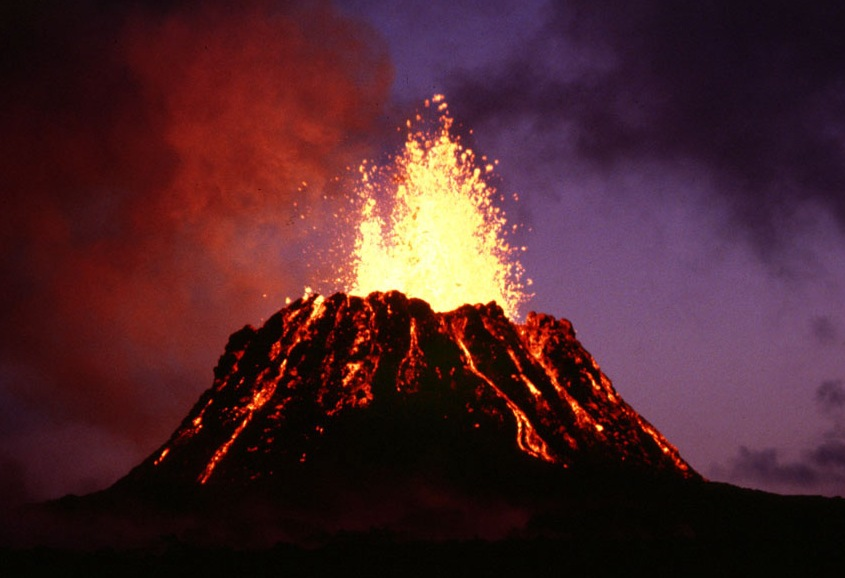
\includegraphics[width=0.55\linewidth]{images/book3/b1-puu-oo-1983.jpg}
\par\smallskip{\small 基拉韦厄火山东裂谷带上的 Pu\textquoteleft
u~\textquoteleft O\textquoteleft o 火山锥上的熔岩喷泉，
1983 年 6 月 29 日，正值持续数十年的喷发之初：
炽热、流动性强的玄武质熔岩，喷射而起，
又落回火山口通道周围。照片：G.~E.~Ulrich，U.S. Geological Survey，公有领域
（维基共享资源）。}
\label{fig:b1:hotspots:puu-oo}
\end{omfigure}
% ledger: commons:puu-oo, pp1801:kilauea-rate

\begin{history}[板块的固定参照系]
1963 年，威尔逊解释了夏威夷群岛：岛屿沿一条线愈来愈老，
其成因是一处岩浆源位于\omterm{def:b1:layered-earth:layers}{地幔}对流环流的缓慢核心中，
而环流较快的上部则将海底带过其上方。
1971 年和 1972 年，摩尔根把该源头定为一根\omterm{def:b1:hotspots:plume}{地幔柱}，
直径约 \qty{150}{km}，从\omterm{def:b1:layered-earth:layers}{地幔}最底部上升，因此
几乎固定不动，而板块在其上方移动；水槽实验很快展示了这种
\omterm{def:b1:hotspots:plume}{地幔柱}的形态。\omterm{def:b1:hotspots:hotspot}{热点}于是成为一个参照系，使板块
可以相对于\omterm{def:b1:layered-earth:layers}{地幔}而非仅相对彼此来测量。半个世纪后，
人们已知该参照系会漂移，夏威夷\omterm{def:b1:hotspots:hotspot}{热点}也在其中，但
漂移得足够缓慢，太平洋的\omterm{def:b1:hotspots:track}{热点轨迹}仍能给出板块相对
\omterm{def:b1:layered-earth:layers}{地幔}的运动，精度为几度与每年几厘米，如本章
的拟合所示。
\end{history}
% ledger: hist:plumes, tarduno:emperor

\section{大火成岩省}\label{sec:b1:hotspots:lips}

\begin{definition}[大火成岩省]\label{def:b1:hotspots:lip}
称\emph{大火成岩省}\index{大火成岩省}（LIP）为
主要由玄武岩组成、非洋中脊正常扩张形成的火成岩堆积，
面积超过 \qty{e5}{km^2}，体积超过
\qty{e5}{km^3}，形成于至多约 5000 万年内，其中大部分
以持续 100 万至 500 万年的脉动形式喷出，这些脉动的
喷出量占其总体积的四分之三以上。陆上大火成岩省多为溢流玄武岩，海洋中则为
海洋高原。
\end{definition}

典型的\omterm{def:b1:hotspots:lip}{大火成岩省}面积约 100 万平方千米，体积约
100 万立方千米熔岩，其中大部分在约 100 万年
或更短时间内喷出。其熔岩呈近乎平坦的层状熔岩流堆叠，侵蚀将其切割成
阶梯，即其名称中的\emph{圈闭}。表中列出了
近 2.6 亿年来的主要\omterm{def:b1:hotspots:lip}{大火成岩省}。
% ledger: be08:definition, cr03:summary

\begin{omfigure}
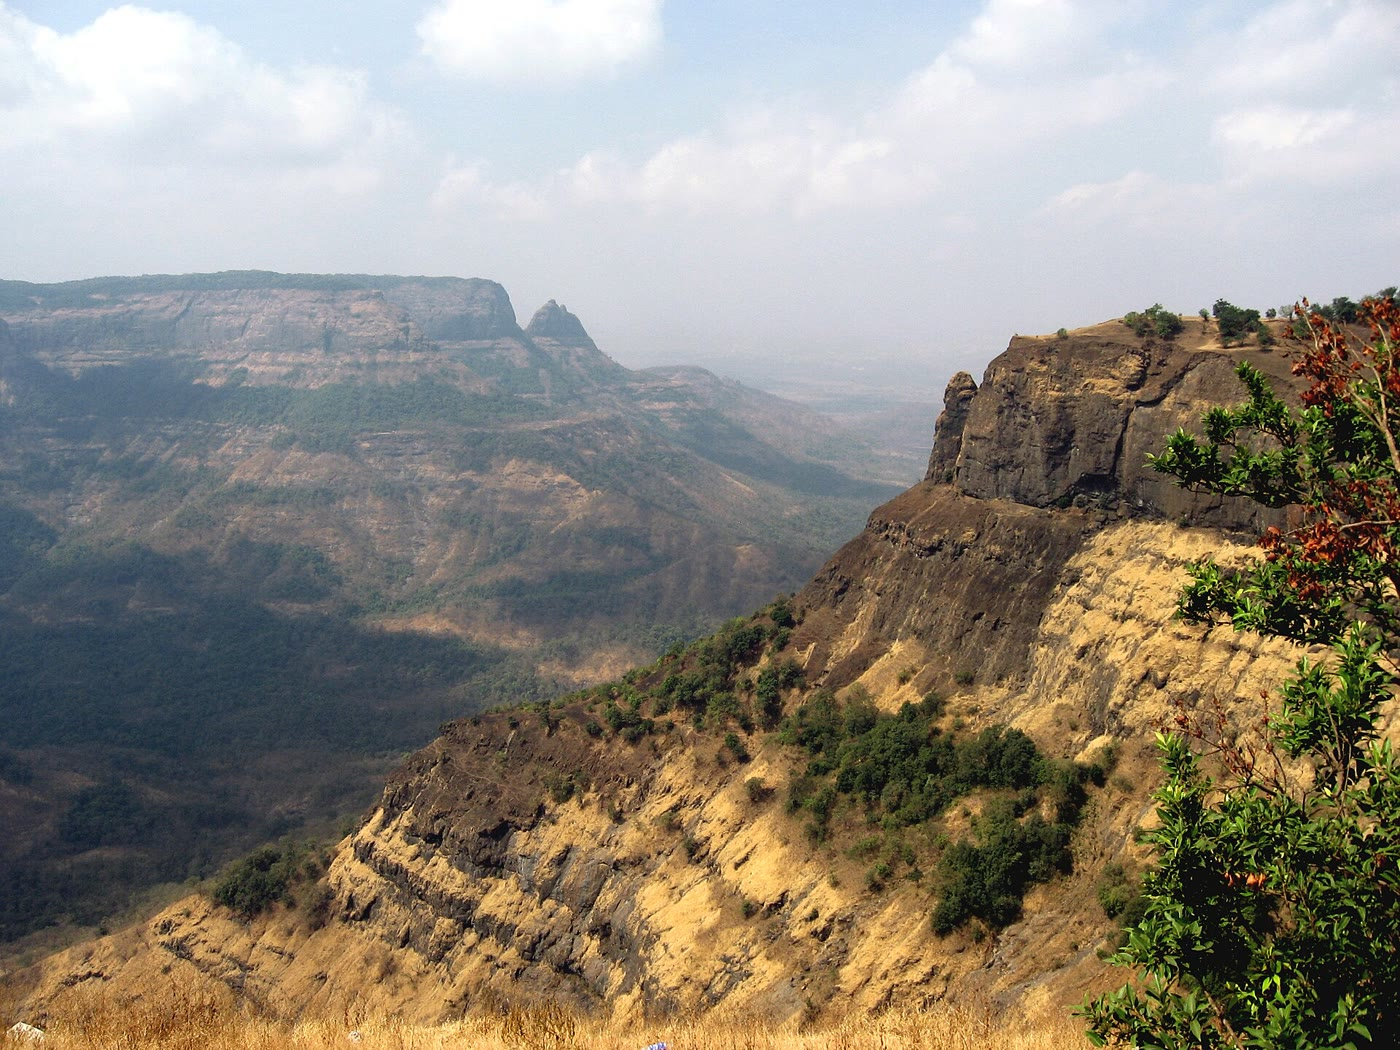
\includegraphics[width=0.55\linewidth]{images/book3/b1-deccan-matheran.jpg}
\par\smallskip{\small 印度马特兰附近的西高止山脉：平顶丘陵
切入德干圈闭中近乎水平的熔岩流堆积，
其抗侵蚀的岩层构成了山坡的阶梯。照片：Nicholas
(Nichalp)，CC BY-SA 2.5（维基共享资源）。}
\label{fig:b1:hotspots:deccan}
\end{omfigure}
% ledger: commons:matheran

\begin{center}
\small
\begin{tabular}{llll}
\hline
岩省 & 年龄（Ma） & 面积（\unit{Mkm^2}） & 初始体积（\unit{Mkm^3}）\\
\hline
哥伦比亚河 & 16 & 0.2 & 0.2\\
埃塞俄比亚–也门 & 30 & 0.7 & 1.2\\
北大西洋 & 61 和 56 & 1.2 & 超过 2\\
德干 & 65.5 & 0.5（曾为 1.8）& 2 至 4\\
翁通爪哇 & 122 和 90 & 2 & 44（整个\omterm{def:b1:layered-earth:layers}{地壳}）\\
巴拉那–埃滕德卡 & 133 & 1.5（曾超过 2）& 超过 2.3\\
卡鲁–法勒 & 183 & 3.1 & 超过 2.5\\
中大西洋（CAMP）& 201 & 曾达 7 & 超过 2\\
西伯利亚圈闭 & 250 & 0.4（曾超过 4）& 超过 3\\
峨眉山 & 259 & 0.5（曾为 2 至 5）& 超过 1\\
\hline
\end{tabular}
\par\smallskip{\small 年龄为平均值；面积取现今值，若有估计则
取初次喷发时的估计值；熔岩体积取初次喷发量，除
翁通爪哇海台外，其数字计入整个加厚的\omterm{def:b1:layered-earth:layers}{地壳}。数据来源：
V.~Courtillot 和 P.~Renne（2003）。}
\end{center}
% ledger: cr03:table

\noindent 在\cref{sec:b1:hotspots:plumes}中勾勒的\omterm{def:b1:hotspots:plume}{地幔柱}模型，兼能解释
规模与速度：直径数百千米的\omterm{def:b1:hotspots:plume}{地幔柱}头抵达
\omterm{def:b1:layered-earth:lithosphere}{岩石圈}底部，减压熔融并漫溢地表；随后
柱尾则继续形成普通的\omterm{def:b1:hotspots:track}{热点轨迹}。若干岩省被认为
位于一条活跃轨迹的老端：德干圈闭与留尼汪
\omterm{def:b1:hotspots:hotspot}{热点}，巴拉那–埃滕德卡与特里斯坦–达库尼亚，由沃尔维斯海岭相连，
以及哥伦比亚河玄武岩与黄石。
% ledger: cr03:deccan (Reunion hot spot, plume-head model), be08:ojmh (Parana-Etendeka-Walvis-Tristan), pm90:track (Columbia River basalts)

印度中西部的德干圈闭是一套熔岩流堆积，厚约
\qty{2500}{m}，其中至少 \qty{1800}{m} 喷发于约
6550 万年前，远不到 100 万年内；今天它们覆盖
约 \qty{0.5}{\mega km^2}，侵蚀前或达 \qty{1.8}{\mega km^2}。
翁通爪哇海台位于西南太平洋，是
所有海洋高原中最大者，面积约 \qty{2}{\mega km^2}，\omterm{def:b1:layered-earth:layers}{地壳}
厚约 \qty{36}{km}，含约 \qty{44}{\mega km^3} 的火成岩。
马尼希基与希库朗伊海台，如今与其相距遥远，之间隔着较年轻的
洋底，可能与之原为同一海台。中大西洋
岩浆省，约于 2.01 亿年前喷发，正值大西洋开始
张开。今天它以熔岩、岩墙与岩床的形式散布于四大陆：
北美洲东部、南美洲东北部、西非与
欧洲西南部。其曾经的覆盖面积可达 \qty{7}{\mega km^2}。
% ledger: cr03:deccan, cr03:table, cr03:ontong-java, be08:ojmh, cr03:camp


若干火成岩省在时间上与生物学所描述的大灭绝相吻合：
西伯利亚暗色岩对应其中规模最大的一次，发生于二叠纪末；
中大西洋岩浆省对应三叠纪末；卡鲁–法勒
省对应早侏罗世的一次灭绝；峨眉山省
对应中二叠世的一次灭绝；德干暗色岩则对应白垩纪末。
过去 2.6 亿年间的四次最大灭绝，各自都
就年代资料所能分辨的精度而言，与其中一个火成岩省相吻合，
并且一种因果联系被认为最有可能。所提出的机制是大气方面的：硫酸盐气溶胶
使气候短期降温，二氧化碳则使其
长期增温，此外还有海洋缺氧。就白垩纪末而言，
德干喷发早于奇克苏鲁布撞击开始，并在撞击之后仍在继续；
一项对该界线记录所作的综述于 2010 年得出结论：
撞击引发了这次灭绝。
% ledger: cr03:table, cr03:summary, cr03:deccan, schulte:kpg

并非所有远离板块边界的火山活动都需要\omterm{def:b1:hotspots:plume}{地幔柱}。小规模火山区
形成于板块被拉伸或开裂之处，而缺乏清晰\omterm{def:b1:hotspots:track}{年龄递进}的
火山链可能由上\omterm{def:b1:layered-earth:layers}{地幔}供给；这正是板块假说在起作用。
\omterm{def:b1:hotspots:hotspot}{热点}离开之后，洋岛会如何演变，
即其下沉、剥蚀并形成礁的过程，属于本科二年级分册。
% ledger: fn03:plate-hypothesis

\section{练习}

\begin{exercise}[$\star$]\label{exo:b1:hotspots:1}
(a) 冒纳凯阿山高出海平面 \qty{4205}{m}，而远离夏威夷海岭的海底
位于 \qty{5274}{m} 深处。该火山高出此海底多少？
它从基底算起的真实高度又为何更大？
(b) 莫纳罗亚火山约含 \qty{74000}{km^3}。堆成此体积需多长时间，
分别按基拉韦厄火山目前的供给速率 \qty{0.1}{km^3} 每年，以及按整条海岭的平均速率，
\qty{0.025}{km^3} 每年计算？(c) 普乌\textquoteleft
u~\textquoteleft O\textquoteleft o 火山喷发在 1983 至 2002 年间每年喷出约 \qty{0.12}{km^3}，
其总量为多少？占莫纳罗亚火山的比例为多少？
% ledger: pp1801:volumes, pp1801:kilauea-supply, pp1801:chain-volume, pp1801:kilauea-rate; 5274 m from hotspots.py
\end{exercise}

\begin{exercise}[$\star$]\label{exo:b1:hotspots:2}
某板块相对于\omterm{def:b1:hotspots:hotspot}{热点}的转动速率为 \qty{0.92}{\degree\per\Ma}。取
$R = \qty{6371}{km}$。(a) 以每百万年的弧度数表示 $\omega$。(b)
计算距极点 \ang{30}、\ang{60}、
\ang{90} 与 \ang{108.0} 处\omterm{def:b1:hotspots:hotspot}{热点}的速度（单位为 \unit{mm.\text{年}^{-1}}）。(c) 为何夏威夷
位于 \ang{108.0} 处时的速度小于位于 \ang{90} 处时的速度？
\end{exercise}

\begin{exercise}[$\star$]\label{exo:b1:hotspots:3}
(a) 计算德干暗色岩今日的平均厚度，
按 \qty{1}{\mega km^3} 除以 \qty{0.5}{\mega km^2}；中大西洋岩浆省的平均厚度则为
即 \qty{2}{\mega km^3} 除以 \qty{7}{\mega km^2}。(b) 与
德干剖面的厚度 \qty{2500}{m} 相比较。(c) 为何中大西洋岩浆省的
平均厚度几乎说明不了其熔岩堆的
厚度？
% ledger: cr03:table, cr03:deccan, cr03:camp
\end{exercise}

\begin{exercise}[$\star$]\label{exo:b1:hotspots:4}
\omterm{def:b1:hotspots:plume}{地幔柱}岩石的温度比周围\omterm{def:b1:layered-earth:layers}{地幔}高 \qty{250}{K}，其
热膨胀系数为 $\alpha = \qty{3.2e-5}{K^{-1}}$，密度为 $\rho_m = \qty{3300}{kg.m^{-3}}$。(a) 它比周围
\omterm{def:b1:layered-earth:layers}{地幔}轻多少（以 \unit{kg.m^{-3}} 计）？(b) 若将这种岩石
铺展于板块之下，要以均衡方式托起海下
高 \qty{690}{m} 的隆起，需多厚的此类岩石？（$\rho_w = \qty{1000}{kg.m^{-3}}$）
% ledger: herzberg:tp (200-300 K), parsons:plate-model (alpha)
\end{exercise}

\begin{exercise}[$\star\star$]\label{exo:b1:hotspots:5}
两个\omterm{def:b1:hotspots:hotspot}{热点}位于赤道上，A 位于东经 \ang{0}，B 位于东经 \ang{90}，两者
的轨迹均正西向（\omterm{def:b1:spherical-astronomy:horizontal}{方位角} \ang{270}）。(a) 计算轨迹矢量
$\vec t_A$ 与 $\vec t_B$。(b) 计算 $\vec t_A\times\vec t_B$。(c) 应用
\cref{prop:b1:hotspots:two-tracks}的符号规则：\omterm{def:b1:plate-kinematics:euler-pole}{欧拉极}位于何处？
不经计算，说明结果。(d) 若 A 以 \qty{50}{mm.\text{年}^{-1}} 运动，
则 $\omega$ 以每百万年的度数计为多少？
\end{exercise}

\begin{exercise}[$\star\star$]\label{exo:b1:hotspots:6}
同一板块上三个\omterm{def:b1:hotspots:hotspot}{热点}距旋转轴的距离分别为 $x = R\sin\Delta = 3000$、5000
与 \qty{6000}{km}，其速度分别为 30、48 与
\qty{57}{mm.\text{年}^{-1}}。(a) 用最小二乘法拟合 $v = \omega x$，
并分别以弧度和每百万年的度数给出 $\omega$。(b) 计算
残差。(c) 为何此直线必须通过原点？
\end{exercise}

\begin{exercise}[$\star\star$]\label{exo:b1:hotspots:7}
一个截面积为 \qty{3e8}{m^2} 的隆起环绕着某板块上的\omterm{def:b1:hotspots:track}{热点轨迹}，该板块
运动速率为 \qty{50}{mm.\text{年}^{-1}}。取 $\rho_m - \rho_w = \qty{2300}{kg.m^{-3}}$，
$c_p = \qty{910}{J.kg^{-1}.K^{-1}}$ 与 $\alpha = \qty{3.2e-5}{K^{-1}}$。(a)
计算其浮力通量与\omterm{def:b1:heat-budget:heat-flow}{热流}量。(b) 与夏威夷的
\qty{3240}{kg.s^{-1}} 相比较。(c) 两个\omterm{def:b1:hotspots:hotspot}{热点}具有相同的隆起，其中一个位于
运动速度快一倍的板块之下。哪一个\omterm{def:b1:hotspots:plume}{地幔柱}更强？
\end{exercise}

\begin{exercise}[$\star\star$]\label{exo:b1:hotspots:8}
沿黄石轨迹，破火山口喷发始于麦克德米特
火山区，约 1610 万年前开始；皮卡博火山区，
位于其东北方约 \qty{350}{km} 处，约 1030 万年前开始；此后，它们
以每年 $\qty[uncertainty-mode=separate]{2.9 \pm 0.5}{cm}$ 的速率向
北偏东 \ang{54}。(a) 火山活动自麦克德米特迁移至
皮卡博的平均速率为多少？(b) 将两者与\omterm{def:b1:hotspots:hotspot}{热点}上方板块的速度
相比较，后者为 \qty[uncertainty-mode=separate]{26 \pm 5}{mm.\text{年}^{-1}}，朝向 \ang{235}。(c) 年轻轨迹的
方向是否符合预期？(d) 轨迹较老的部分
位于火山活动经过之后被拉伸的区域。
这能否解释二者的差异？
% ledger: pm90:track, data:b3-hotspots
\end{exercise}

\begin{exercise}[$\star\star$]\label{exo:b1:hotspots:9}
夏威夷\omterm{def:b1:hotspots:plume}{地幔柱}携带约 \qty{9.2e10}{W} 的过剩热量。(a) 若其全部
经由最靠近\omterm{def:b1:hotspots:hotspot}{热点}的 \qty{1000}{km} × \qty{1000}{km} 海底散失，
则该处\omterm{def:b1:heat-budget:heat-flow}{热流}将升高多少？(b) 与
观测到的过剩值相比较，后者至多为 5 至 \qty{10}{mW.m^{-2}}。(c) 热量
需多长时间才能在厚 \qty{100}{km} 的板块中扩散（$\kappa = \qty{e-6}{m^2.s^{-1}}$）？
板块以 \qty{92}{mm.\text{年}^{-1}} 的速度穿越 \qty{1000}{km} 需多长时间？
试作出结论。
% ledger: vh89:swell-heat
\end{exercise}

\begin{exercise}[$\star\star\star$]\label{exo:b1:hotspots:10}
德干玄武岩省约含 \qty{e6}{km^3} 的熔岩。假设其来自一个
球形\omterm{def:b1:hotspots:plume}{地幔柱}头，其中十分之一熔化。(a) 该柱头的体积与
半径分别为多少？(b) 若将其在\omterm{def:b1:layered-earth:lithosphere}{岩石圈}下方压平成一个
厚 \qty{100}{km} 的圆盘，则柱头直径为多少？将其面积与
德干玄武岩省可能曾覆盖的面积 \qty{1.8}{\mega km^2} 相比较。(c) 若
熔岩在一百万年内喷发，则将其速率与基拉韦厄火山当前的
补给量（\qty{0.1}{km^3} 每年）相比较。(d) 为何\omterm{def:b1:hotspots:plume}{地幔柱}头必须很大，
而其后的柱尾却很窄？
% ledger: cr03:table, pp1801:kilauea-supply
\end{exercise}

\begin{exercise}[$\star\star\star$]\label{exo:b1:hotspots:11}
在 8100 万至 4700 万年前，夏威夷\omterm{def:b1:hotspots:hotspot}{热点}以超过
\qty{40}{mm.\text{年}^{-1}} 的速率向南移动。(a) 取 \qty{40}{mm.\text{年}^{-1}}，它
移动了多远？
(b) 设同期板块以 \qty{80}{mm.\text{年}^{-1}} 的速率朝
\ang{340} 方向在深部\omterm{def:b1:layered-earth:layers}{地幔}上运动。取 $x$ 向东、$y$ 向北，计算
板块相对漂移\omterm{def:b1:hotspots:hotspot}{热点}的速度矢量、其速率与其
\omterm{def:b1:spherical-astronomy:horizontal}{方位角}。(c) 该时段形成的轨迹，对板块在深部\omterm{def:b1:layered-earth:layers}{地幔}上运动的歪曲
分别有多大（以百分比和度数计）？
% ledger: tarduno:emperor
\end{exercise}

\begin{exercise}[$\star\star\star$]\label{exo:b1:hotspots:12}
(a) 体积为 \qty{e6}{km^3} 的溢流玄武岩自约 \qty{1300}{\celsius} 冷却至
地表温度。取热容为 \qty{3}{MJ.m^{-3}.K^{-1}}，
放出多少热量（忽略结晶潜热）？
(b) 若分摊在一百万年内，其功率为多少？与
夏威夷\omterm{def:b1:hotspots:plume}{地幔柱}的 \qty{9.2e10}{W}，以及全地球的 \qty{47}{TW} 相比较。
(c) \omterm{def:b1:hotspots:plume}{地幔柱}头还会加\omterm{def:b1:heat-budget:boundary-layer}{热岩石圈}底部，却不使其全部
熔化。(b) 的功率对柱头所带热量而言，是上界还是
下界？
% ledger: delaney86:properties (Book 2 row, 2-3 MJ/m3/K), dd10:total; 1300 degC is an exercise value
\end{exercise}

\section{问题：太平洋板块的速度计}

\begin{problem}[{周末问题——由两条热点轨迹求太平洋板块的欧拉极，
由第三次测量求其速率，对其他热点的检验，
以及夏威夷地幔柱的浮力与供应}]
\label{pb:b1:hotspots:1}
% values: calc/ch15.py; ledger: data:b3-hotspots, data:etopo1, pp1801:kilauea-supply, pp1801:volumes,
% pp1801:chain-volume, delaney86:properties, parsons:plate-model, dd10:total, data:pb2002 (ridge_budget.py), cd87:rate
摩尔根和摩尔根给出夏威夷\omterm{def:b1:hotspots:hotspot}{热点}位于北纬 \ang{19.0}，西经 \ang{155.2}，
轨迹指向 $\ang{304}\pm\ang{3}$，速率为
\qty[uncertainty-mode=separate]{92 \pm 3}{mm.\text{年}^{-1}}，而路易斯维尔\omterm{def:b1:hotspots:hotspot}{热点}
位于南纬 \ang{53.6}，西经 \ang{140.6}，轨迹指向 $\ang{316}\pm\ang{5}$，
速率为 \qty[uncertainty-mode=separate]{67 \pm 5}{mm.\text{年}^{-1}}。
取\cref{sec:b1:hotspots:tracks}中的坐标轴与矢量 $\vec e$、$\vec n$、$\vec t$，
其中 $R = \qty{6371}{km}$。
分量取到小数点后四位。

\medskip
\noindent\textbf{第一部分——由两条轨迹求极点。}
\begin{enumerate}
  \item 在夏威夷计算 $\vec r$、$\vec e$ 和 $\vec n$，再求
        轨迹矢量 $\vec t_H$。
  \item 在路易斯维尔同样计算 $\vec r_L$、$\vec e$、$\vec n$，再求
        轨迹矢量 $\vec t_L$。
  \item 验证 $\vec t_H$ 为与 $\vec r_H$ 垂直的单位矢量。
  \item 计算 $\vec t_H\times\vec t_L$ 及其长度。
        两条轨迹矢量的夹角是多少？
  \item 将叉积单位化，并应用
        \cref{prop:b1:hotspots:two-tracks}中的符号规则。
  \item 给出太平洋板块相对\omterm{def:b1:hotspots:hotspot}{热点}的\omterm{def:b1:plate-kinematics:euler-pole}{欧拉极}的
        \omterm{def:b1:spherical-astronomy:geographic}{纬度}与\omterm{def:b1:spherical-astronomy:geographic}{经度}。
\end{enumerate}

\medskip
\noindent\textbf{第二部分——速率。}
\begin{enumerate}[resume]
  \item 计算由极点到两个\omterm{def:b1:hotspots:hotspot}{热点}的角距离
        $\Delta_H$ 与 $\Delta_L$。
  \item 计算 $(\vec p\times\vec r_L)\cdot\vec t_L$，说明其为何等于
        $\sin\Delta_L$，并说明其符号对路易斯维尔处的运动说明了什么。
  \item 由路易斯维尔处的速率，以弧度和
        度每百万年为单位计算 $\omega$。
  \item 太平洋板块绕该极旋转一整圈需
        多长时间？
  \item 十五条太平洋轨迹的最小二乘极位于
南纬 \ang{63.78}，东经 \ang{112.48}，速率为 \qty{0.92}{\degree\per\Ma}。
        计算两极之间的夹角，并比较两者的速率。
\end{enumerate}

\medskip
\noindent\textbf{第三部分——对另外三个\omterm{def:b1:hotspots:hotspot}{热点}的检验。}摩尔根和摩尔根
给出社会群岛\omterm{def:b1:hotspots:hotspot}{热点}（南纬 \ang{18.2}，西经 \ang{148.4}）
\qty[uncertainty-mode=separate]{109 \pm 10}{mm.\text{年}^{-1}}，皮特凯恩\omterm{def:b1:hotspots:hotspot}{热点}
（南纬 \ang{25.4}，西经 \ang{129.3}）
\qty[uncertainty-mode=separate]{90 \pm 15}{mm.\text{年}^{-1}}，以及科布
\omterm{def:b1:hotspots:hotspot}{热点}（北纬 \ang{46.0}，西经 \ang{130.1}）
\qty[uncertainty-mode=separate]{43 \pm 3}{mm.\text{年}^{-1}}。
\begin{enumerate}[resume]
  \item 计算第 6 题中的极点到三个\omterm{def:b1:hotspots:hotspot}{热点}各自的
        角距离。
  \item 用第 9 题的速率预测三个\omterm{def:b1:hotspots:hotspot}{热点}的速度。
  \item 哪些预测值与实测速度在各自的不确定度范围内相符，
        哪些不相符？
  \item 两条方向不同的轨迹总能确定一个极点。为何两条
        近乎平行的轨迹是较差的选择？
\end{enumerate}

\medskip
\noindent\textbf{第四部分——\omterm{def:b1:hotspots:plume}{地幔柱}与速度计。}夏威夷海底隆起
的截面为 \qty{4.83e8}{m^2}。取
$\rho_m - \rho_w = \qty{2300}{kg.m^{-3}}$，$c_p = \qty{910}{J.kg^{-1}.K^{-1}}$
以及 $\alpha = \qty{3.2e-5}{K^{-1}}$。
\begin{enumerate}[resume]
  \item 将 \qty{92}{mm.\text{年}^{-1}} 换算为 \unit{m.s^{-1}}，并计算
        夏威夷\omterm{def:b1:hotspots:plume}{地幔柱}的浮力通量。
  \item 计算其携带的过剩热量，并与地球散失的
        \qty{47}{TW} 相比较。
  \item 洋中脊沿某些总长约
        \qty{67000}{km} 的部分每年生成约 \qty{21}{km^3} 的\omterm{def:b1:layered-earth:layers}{地壳}。
        需要多长的洋中脊，才能生成与基拉韦厄火山每年获得补给 \qty{0.1}{km^3} 同样多的\omterm{def:b1:layered-earth:layers}{地壳}？
  \item 按此速率，体积约 \qty{74000}{km^3} 的莫纳罗亚火山需要
        多长时间才能长成？
  \item 该\omterm{def:b1:hotspots:hotspot}{热点}在 8100 万年内形成了约 \qty{2e6}{km^3} 的海山链，
        计算其平均产出，并与基拉韦厄火山当前的补给量相比较。
  \item 利用第一、二部分求得的极点与速率，计算路易斯维尔轨迹
        所预测的太平洋板块相对夏威夷\omterm{def:b1:hotspots:hotspot}{热点}的
        速度。
  \item 与实测值 \qty[uncertainty-mode=separate]{92 \pm 3}{mm.\text{年}^{-1}} 相比较：二者相差多少，
        相差几个标准不确定度？
  \item 根据夏威夷火山的年龄，第 2 册得出
        \qty{9.1}{cm} 每年；年龄数据的作者们拟合整条海山链后得出
        \qty{8.6}{cm} 每年。比较这些在数千万年尺度上的平均值
        与两个\omterm{def:b1:hotspots:hotspot}{热点}的速度。
  \item 以厘米每年为单位，保留一位小数，路易斯维尔
        轨迹给出的太平洋板块相对夏威夷\omterm{def:b1:hotspots:hotspot}{热点}的速度是多少？
\end{enumerate}
\end{problem}
